
\chapter{Preview import}

La finestra preview import permette
di importare una serie di registri precedentemente esportati
in modo da inviarli in blocco allo slave modbus.
La finestra di import può essere aperta dal menu "import", 
tramite il pulsante import in basso oppure premendo il tasto
dx sulle tabelle della finestra principale:

\begin{figure}[H]
\centering
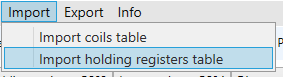
\includegraphics[width=0.35\textwidth]{../Img/Menu_Import.PNG}
\caption{Preview import}
\end{figure}

\begin{figure}[H]
\centering
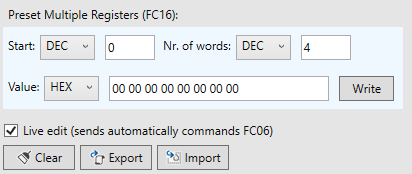
\includegraphics[width=0.35\textwidth]{../Img/PreviewImport_OpenButton.PNG}
\caption{Preview import}
\end{figure}

\begin{figure}[H]
\centering
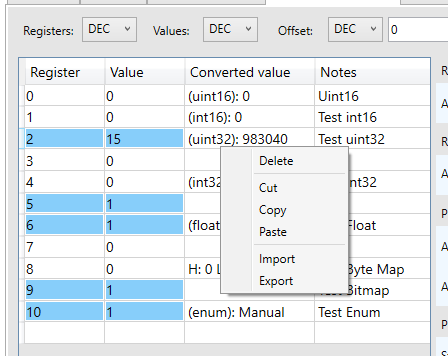
\includegraphics[width=0.50\textwidth]{../Img/PreviewImport_Open.PNG}
\caption{Preview import}
\end{figure}

Dal menu contestuale è possibile sia importare una serie di registri
copiati da un foglio di calcolo ("paste") sia importare un file
.csv/.json ("import"). I comandi "copy" o "cut" permettono di copiare 
la tabella visualizzata nella clipboard e incollarle poi in un foglio di calcolo.

\newpage
La finestra preview si presenta come segue:

\begin{figure}[H]
\centering
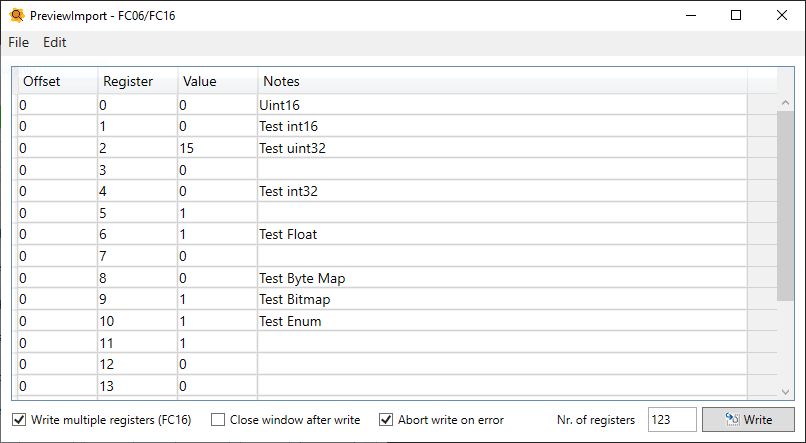
\includegraphics[width=0.85\textwidth]{../Img/PreviewImport_Main.PNG}
\caption{Preview import finestra principale}
\end{figure}

I dati visualizzati nella preview possono essere copiati o incollati
nella finestra tramite il menu contestuale:

\begin{figure}[H]
\centering
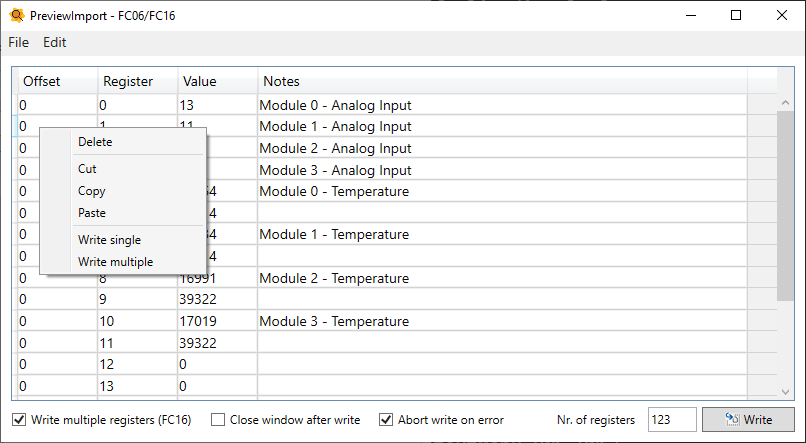
\includegraphics[width=0.85\textwidth]{../Img/PreviewImport_ContextMenu.PNG}
\caption{Preview import menu contestuale}
\end{figure}

I comandi "write single" e "write multiple" permettono di inviare
i registri visualizzati in gruppo (FC15/FC16) o singolarmente (FC05/FC06).



